\documentclass[10pt,a4paper,twocolumn]{article}
% First draft. Replace preamble/layout with the instructor's template when received.
\usepackage[margin=1.8cm,columnsep=0.7cm]{geometry}
\usepackage[T1]{fontenc}
\usepackage{lmodern}
\usepackage{amsmath,amssymb}
\usepackage{booktabs}
\usepackage{graphicx}
\usepackage{xcolor}
\usepackage[round,authoryear]{natbib}
\usepackage{xurl}
\usepackage[colorlinks=true,citecolor=blue!50!black,linkcolor=blue!50!black,urlcolor=blue!50!black]{hyperref}
\usepackage{caption}
\usepackage{adjustbox}
\usepackage{tikz}
\usetikzlibrary{positioning,arrows.meta}
\captionsetup{font=small,labelfont=bf}
\graphicspath{{figures/}}

% Placeholder marker for content that needs human input or pending pipeline output.
\newcommand{\todo}[1]{\textcolor{red}{[\textbf{TODO:} #1]}}
\newcommand{\INR}{\ensuremath{\text{\rupee}}}
\renewcommand{\INR}{INR~}

% Every number in the text comes from the pipeline (scripts/export_numbers.py).
% Generated by scripts/export_numbers.py -- do not edit
\newcommand{\AreaKm}{720}
\newcommand{\NDemandCells}{3,426}
\newcommand{\NOsmSites}{1,480}
\newcommand{\NCandidates}{1,133}
\newcommand{\PopWorldPop}{6.04}
\newcommand{\Detour}{1.57}
\newcommand{\DetourLo}{1.41}
\newcommand{\DetourHi}{1.81}
\newcommand{\KaggleOffsetPct}{98.4}
\newcommand{\CurrentStores}{440}
\newcommand{\BaseV}{15}
\newcommand{\BaseT}{15}
\newcommand{\StoresTTen}{320}
\newcommand{\CostPerOrderTen}{43.4}
\newcommand{\ServedTenPct}{86.7}
\newcommand{\RidersTen}{6,902}
\newcommand{\StoresTFifteen}{240}
\newcommand{\CostPerOrderFifteen}{43.2}
\newcommand{\ServedFifteenPct}{98.3}
\newcommand{\RidersFifteen}{9,275}
\newcommand{\StoresTTwenty}{239}
\newcommand{\CostPerOrderTwenty}{43.9}
\newcommand{\ServedTwentyPct}{99.9}
\newcommand{\RidersTwenty}{9,700}
\newcommand{\StoresTThirty}{238}
\newcommand{\CostPerOrderThirty}{43.9}
\newcommand{\ServedThirtyPct}{100.0}
\newcommand{\RidersThirty}{9,733}
\newcommand{\UnreachTenPct}{13.3}
\newcommand{\CostPerOrderVTwelve}{49.3}
\newcommand{\CostPerOrderVTwenty}{36.3}
\newcommand{\SpeedCapPremiumPct}{19}
\newcommand{\StoreRange}{202--390}
\newcommand{\PertTenP}{99.7}
\newcommand{\PertTenSpeed}{12.1}
\newcommand{\AssignStressTenOnTime}{64}
\newcommand{\AssignStressSpeed}{20}
\newcommand{\AssignStressRide}{1.3}
\newcommand{\TransLP}{5.80}
\newcommand{\TransVAM}{5.85}
\newcommand{\TransNW}{13.29}
\newcommand{\TransNearest}{5.60}
\newcommand{\TransVAMGapPct}{0.9}
\newcommand{\TransNWRatio}{2.3}
\newcommand{\TransCapPremiumPct}{3.5}
\newcommand{\GridTenStores}{462}
\newcommand{\GridTenServedPct}{100.0}
\newcommand{\GridTenCost}{45.9}
\newcommand{\GridFifteenStores}{287}
\newcommand{\GridFifteenCost}{42.4}
\newcommand{\GridStorePremiumPct}{61}
\newcommand{\GridCostPremiumPct}{8.4}
\newcommand{\GridPricePerMinute}{0.71}
\newcommand{\GridCandidates}{860}
\newcommand{\TornadoTop}{rider cost}
\newcommand{\TornadoSecond}{rider utilisation}
\newcommand{\TornadoTopSpan}{13.4}
\newcommand{\TornadoSecondSpan}{11.0}
\newcommand{\FragTenOne}{74.6}
\newcommand{\FragFifteenOne}{98.3}
\newcommand{\FragTenMax}{86.7}
\newcommand{\FragFifteenHundred}{98.1}
\newcommand{\MixedStores}{318}
\newcommand{\MixedTenShare}{86.7}
\newcommand{\MixedServed}{98.3}
\newcommand{\MixedCost}{45.0}
\newcommand{\MixedPremiumPct}{4.2}
\newcommand{\MixedExtraStores}{78}
\newcommand{\NMilps}{29}
\newcommand{\NMilpsOptimal}{27}
\newcommand{\NMilpsLimit}{2}
\newcommand{\MaxSolveS}{154}

% Generated by scripts/build_lit_assets.py -- do not edit
\newcommand{\BibIdentified}{7,576}
\newcommand{\BibAfterMethod}{715}
\newcommand{\BibScreened}{216}
\newcommand{\BibIncluded}{168}
\newcommand{\BibExcluded}{48}
\newcommand{\BibExclScope}{37}
\newcommand{\BibExclNoOR}{10}
\newcommand{\BibExclIntro}{1}
\newcommand{\BibSearchDate}{2026-10-06}
\newcommand{\BibGrowthPct}{31.4}
\newcommand{\BibSinceTwentyOnePct}{91}
\newcommand{\BibYearsTwentyFive}{46}
\newcommand{\BibTopJournal}{European Journal of Operational Research}
\newcommand{\BibTopJournalN}{20}
\newcommand{\BibSecondJournal}{Computers \& Operations Research}
\newcommand{\BibSecondJournalN}{14}
\newcommand{\BibDrones}{54}
\newcommand{\BibAssign}{50}
\newcommand{\BibLocation}{23}
\newcommand{\BibOnDemand}{27}
\newcommand{\BibQComm}{3}
\newcommand{\BibIndia}{0}
\newcommand{\BibWelfare}{4}
\newcommand{\BibPromise}{4}
\newcommand{\BibReviews}{9}
\newcommand{\BibMILPKw}{49}
\newcommand{\BibALNSKw}{17}


\title{The Price of Speed: Optimising Dark-Store Networks and Rider Assignment under Relaxed Delivery Promises in Indian Quick Commerce}
\author{\small\setlength{\tabcolsep}{7pt}\begin{tabular}{cccccc}Madhav Gupta & Aadee Pardasani & Aashi Khuthia & Jiya Jagawat & Prishi Doshi & Aarushi Rakesh \\ {\footnotesize Roll No.\ 28} & {\footnotesize Roll No.\ 01} & {\footnotesize Roll No.\ 06} & {\footnotesize Roll No.\ 23} & {\footnotesize Roll No.\ 36} & {\footnotesize Roll No.\ 05}\end{tabular}}
\date{October 2026}

\begin{document}
\twocolumn[\maketitle\vspace{-1em}\begin{abstract}
In January 2026 India's quick-commerce platforms withdrew their ``10-minute delivery'' claims after the Union Labour Ministry raised rider-safety concerns, and in August 2026 a Parliamentary Standing Committee recommended curbs on ``unrealistic speed targets'' without defining them. We combine a bibliometric review of operations research on last-mile and on-demand delivery \todo{N articles, 2015--2026} with an integrated optimisation model of a Bengaluru dark-store network built entirely from public data: WorldPop 2025 population, BBMP ward boundaries, OpenStreetMap retail sites and operating metrics from listed platforms' shareholder letters. A coverage-constrained facility-location model opens stores and allocates demand at minimum store and rider cost while guaranteeing a promise $T$ at a safe rider speed $v$; a transportation model plans replenishment, an assignment model dispatches riders at peak, and a PERT model estimates on-time probability. At \BaseV~km/h, the cost-optimal network has about \StoresTFifteen{} stores and reaches \ServedFifteenPct\% of residents for any promise of 15 minutes or more; with the available retail sites a 10-minute promise needs \StoresTTen{} stores and still leaves \UnreachTenPct\% unreachable. Serving everyone within 10 minutes requires \GridStorePremiumPct\% more stores and \GridCostPremiumPct\% higher cost per order than within 15 minutes. Rider speed, not the promise, drives cost: capping speed at 15 rather than 20~km/h raises cost per order by about \SpeedCapPremiumPct\%. Asking a 15-minute network to deliver in 10 minutes meets the promise for only \AssignStressTenOnTime\% of orders at a stressed store unless riders exceed safe speeds. We propose reachability within a safe ride radius as an operational definition of a ``realistic'' promise.

\medskip\noindent\textbf{Keywords:} quick commerce; dark stores; facility location; transportation problem; assignment problem; PERT; bibliometric analysis; gig-worker safety; India
\end{abstract}
\vspace{1em}]
\section{Introduction}\label{sec:intro}

Quick commerce (q-commerce) promises groceries and household essentials within minutes, fulfilled from small urban warehouses called \emph{dark stores}. India has become its largest laboratory: in the April--June 2026 quarter Blinkit alone reported 2,443 dark stores and 331 million orders \citep{eternal2026q1}, and Swiggy Instamart a further 1,171 stores \citep{swiggy2026q1}. The model rests on a simple geometry: a store that serves only a 1.5--3~km radius can meet a 10-minute promise without riders travelling fast, which is how platform founders defended it \citep{palicha2022,dhindsa2021}.

That defence has been tested. After a nationwide strike by gig workers on 31 December 2025, the Union Labour Ministry intervened and in January 2026 Blinkit, Zepto, Swiggy Instamart and Zomato dropped ``10-minute delivery'' from their branding \citep{outlook2026drop}. In August 2026 the Parliamentary Standing Committee on Commerce recommended guidelines against ``unrealistic speed targets'' set by dispatch algorithms, but did not say what makes a target unrealistic \citep{outlook2026panel}. The policy debate therefore lacks a quantitative answer to a classical OR question: \emph{what does each minute of delivery promise cost, and who pays for it---the platform, through more stores, or the rider, through higher speed?}

This paper answers that question for Bengaluru, India's most contested q-commerce market, and situates it in the OR literature. We pose three research questions:

\begin{description}
  \item[RQ1] How has OR research on on-demand and last-mile delivery evolved, which methods dominate (location, assignment, routing), and where are the gaps for quick commerce and courier welfare?
  \item[RQ2] For Bengaluru, how do the number of dark stores, rider requirements and cost change as the delivery promise relaxes from 10 to 15, 20 and 30 minutes under a safety-capped rider speed?
  \item[RQ3] Which promise level and network design balance coverage, cost and rider safety, and what does this imply for defining a ``realistic'' speed target?
\end{description}

Our contributions are fourfold. First, a bibliometric map of OR research on last-mile and on-demand delivery from 2015 to 2026, which shows a fast-growing field (\BibGrowthPct\% a year) centred on vehicle routing with new delivery modes, in which only \BibQComm{} of \BibIncluded{} articles address quick commerce, none studies India and only \BibWelfare{} consider courier welfare. Second, an integrated and fully reproducible model chain---coverage-constrained facility location, transportation, assignment and PERT---built from public Indian data, together with an audit showing why widely used Kaggle delivery datasets are unsuitable for spatial modelling. Third, a ``price of speed'' curve for Bengaluru. Fourth, evidence for regulators on where a delivery promise stops being achievable through network design and starts depending on rider speed.

Section~\ref{sec:lit} reviews the literature; Section~\ref{sec:method} describes the bibliometric protocol and modelling framework; Section~\ref{sec:data} presents the case and data; Section~\ref{sec:model} formulates the models; Section~\ref{sec:results} reports results; Section~\ref{sec:discussion} discusses implications and limitations; Section~\ref{sec:conclusion} concludes.

\section{Literature review}\label{sec:lit}

% Draft structure. Bibliometric numbers and figures are produced by biblio/R/02_analysis.R
% once the EBSCO search and screening are complete (PLAN.md Phases 2-3).

\subsection{Bibliometric overview}

\todo{Run the EBSCO search (Section~\ref{sec:method}); report records identified, screened and included, the annual growth rate, leading journals, authors and countries, and insert Figures: annual production, keyword co-occurrence network, thematic map (biblio/figures/).}

\subsection{Thematic synthesis}

We organise the core studies into four streams. \todo{Confirm the clusters against the Biblioshiny thematic map and add 10--20 core papers from the screened library.}

\paragraph{Last-mile delivery and its operating modes.} Research on urban last-mile logistics spans vehicle routing variants, parcel lockers, micro-depots, crowdshipping and electric fleets; recent bibliometric reviews document rapid growth and a strong sustainability orientation \todo{cite EV last-mile and crowdshipping bibliometric reviews from the library}.

\paragraph{On-demand and meal delivery operations.} The meal delivery routing problem \citep{reyes2018mdrp} framed courier assignment and dispatch under tight delivery windows as a dynamic pickup-and-delivery problem, and a substantial literature on order--courier matching followed \todo{cite reviews, e.g.\ on-demand food delivery SLR; MSOM data paper}. These studies typically treat the promised delivery time as given, not as a design choice.

\paragraph{Facility location for urban fulfilment.} Covering models originate with the location set covering problem \citep{toregas1971} and the maximal covering location problem \citep{church1974}. Recent work adapts them to micro-fulfilment and dark stores: \citet{kewalramani2023} propose a heuristic for dark-store siting under delivery-radius and capacity constraints for an Indian q-commerce operator, and \todo{cite TUM/Augsburg micro-fulfilment network planning; dark-store resilience MILP}.

\paragraph{Courier welfare in OR.} \todo{Expected to be thin: report what the search finds. Fairwork India ratings document pay and safety conditions outside the OR literature.}

\subsection{Research gaps}

Three gaps motivate this study: (i) quick commerce in India has received little OR attention relative to its scale; (ii) the delivery promise is almost always an exogenous parameter rather than a policy variable to be priced; and (iii) rider safety enters models, if at all, as a by-product rather than a constraint. \todo{Ground each gap in the bibliometric evidence.}

\section{Research methodology}\label{sec:method}

\subsection{Bibliometric data collection}

Following the course protocol, we searched EBSCOhost academic journals in English published between 2015 and 2026 with the Boolean string
\begin{quote}\footnotesize\ttfamily\raggedright
"operations" AND "research" AND ("last-mile" OR "last mile" OR "on-demand delivery" OR "instant delivery" OR "quick commerce" OR "q-commerce" OR "meal delivery" OR "dark store" OR "micro-fulfil*" OR "crowdshipping") AND ("facility location" OR "covering" OR "assignment" OR "vehicle routing" OR "integer programming" OR "linear programming")
\end{quote}
\todo{date executed; records identified; screening counts; PRISMA figure from scripts/prisma.py; exclusion reasons.} Records were exported in RIS format, de-duplicated and verified in Mendeley, and analysed with the Bibliometrix R package \citep{aria2017bibliometrix}; citation counts were taken from Google Scholar \todo{retrieval date}.

\subsection{Modelling framework}

The case study links four classical OR models at three planning levels (Figure~\ref{fig:chain}). Strategically, a coverage-constrained facility-location model (M1) opens dark stores and allocates demand so that every served household is reachable within the promise $T$ at a safe rider speed $v$, at minimum store and rider cost; rider requirements follow from cycle times (M2). Tactically, a transportation model (M3) plans daily replenishment from mother hubs to the chosen stores. Operationally, an assignment model (M4) dispatches riders to orders in a peak batch, and a PERT model (M5) converts the variability of picking, dispatch and riding into the probability that an order meets $T$. The promise $T$ and speed $v$ are swept as policy parameters; everything else is calibrated from public sources (Section~\ref{sec:data}).

\begin{figure}[ht]
\centering\small
\fbox{\parbox{0.92\linewidth}{\centering
\textbf{Policy inputs:} promise $T$, safe speed $v$ \quad$\Rightarrow$\quad
\textbf{M1} store location + allocation (MILP) \quad$\Rightarrow$\quad \textbf{M2} rider sizing\\[3pt]
$\Downarrow$ open stores \hspace{4cm} $\Downarrow$ store loads, ride distances\\[3pt]
\textbf{M3} replenishment (transportation LP) \qquad \textbf{M4} peak dispatch (assignment IP) \qquad \textbf{M5} on-time probability (PERT)
}}
\caption{Model chain. \todo{Replace with a proper diagram.}}
\label{fig:chain}
\end{figure}

All models are implemented in Python with PuLP and solved with HiGHS; code, data provenance and a test suite verifying each model against hand-solvable or brute-force instances are available in the project repository \todo{repo link}.

\section{Case and data}\label{sec:data}

\subsection{Study area}

The study area is the Bruhat Bengaluru Mahanagara Palike (BBMP) as delimited into 243 wards in 2022 \citep{opencity2022wards}; the ward polygons cover \AreaKm~km\textsuperscript{2}, consistent with the official 712.5~km\textsuperscript{2}. Bengaluru hosts roughly \CurrentStores{} dark stores of the three largest platforms \citep{qcmap2026}, making it the most contested q-commerce market in India.

\subsection{Data sources and audit}

Table~\ref{tab:sources} lists the inputs. Demand is spatialised with the WorldPop 2025 constrained population grid at 100~m \citep{worldpop2025}, aggregated to \NDemandCells{} cells of about 0.46~km. WorldPop sums to \PopWorldPop~million inside BBMP---below the 2011 Census count of 8.44 million \citep{census2011}---because it caps density in the dense core; we therefore keep its spatial pattern and scale it to the census total. Candidate store sites are the \NOsmSites{} supermarkets, grocery and convenience shops and warehouses mapped in OpenStreetMap within BBMP \citep{osm2026}, merged into \NCandidates{} candidate locations. Road distances are straight-line distances multiplied by a detour factor of \Detour{} (interquartile range \DetourLo--\DetourHi), the median road/straight-line ratio over a random sample of OSRM routes.

\begin{table*}[t]
\centering\small
\caption{Data sources.}\label{tab:sources}
\begin{tabular}{p{0.20\linewidth}p{0.40\linewidth}p{0.28\linewidth}}
\toprule
Input & Source & Use \\
\midrule
Population & WorldPop R2025A, India 2025, 100~m constrained & Spatial demand weights \\
Boundary & BBMP ward map 2022 (OpenCity) & Study area \\
Candidate sites & OpenStreetMap, Geofabrik extract 2026-10-05 & Possible dark stores \\
Road detour & OSRM, OSM road network & Distance correction \\
Orders, stores, costs & Eternal and Swiggy shareholder letters Q1~FY27; press & Calibration (Table~\ref{tab:params}) \\
\bottomrule
\end{tabular}
\end{table*}

Two popular Kaggle datasets on Indian food and grocery delivery were evaluated and rejected. In the food-delivery dataset, \KaggleOffsetPct\% of delivery points equal the restaurant coordinates plus an identical latitude--longitude offset drawn from 13 values, and road-traffic level is fully determined by the hour of day; the delivery geometry and timing are synthetic. The Blinkit sales dataset uses placeholder e-mail domains for all customers. Neither can support distance-based modelling, a caution for the many studies that use them.

\subsection{Parameters}

Table~\ref{tab:params} summarises the calibration. Bengaluru demand is estimated as stores per platform times orders per store per day: Blinkit \citep[derived from net order value per store per day and average order value]{eternal2026q1}, Swiggy Instamart \citep[1,089 orders per store per day]{swiggy2026q1} and Zepto (mean of the two), giving about 600,000 orders per day. Rider cost uses the average of INR~102 per logged-in hour reported by Eternal for 2025 \citep{goyal2026earnings}. Speeds and pick-pack times follow statements by platform founders \citep{palicha2022,dhindsa2021}. As a validation, the implied rider cost per order in the base case falls within the reported per-order pay of INR~25--35.

\begin{table*}[t]
\centering\small
\caption{Model parameters (base value and sensitivity range).}\label{tab:params}
\begin{tabular}{p{0.28\linewidth}p{0.22\linewidth}p{0.38\linewidth}}
\toprule
Parameter & Base (range) & Basis \\
\midrule
Delivery promise $T$ & 10, 15, 20, 30 min & Policy scenarios \\
Safe rider speed $v$ & 15 (12--20) km/h & \citet{palicha2022} \\
Pick + pack (PERT $a,m,b$) & 1.3, 2, 4 min & \citet{dhindsa2021}; Zepto 76~s \\
Rider assignment; handover & (0, 0.5, 2); (0.5, 1, 2) min & Assumption \\
Daily orders, Bengaluru & 600k (450k--750k) & \citet{eternal2026q1,swiggy2026q1,qcmap2026} \\
Peak-hour share of daily orders & 0.10 (0.08--0.12) & Assumption (evening peak) \\
Store fixed cost & INR 8 (6--11) lakh/month & Opex + capex/60 months \\
Rider cost & INR 125 (102--154)/h & \citet{goyal2026earnings} \\
Rider utilisation & 0.6 (0.5--0.7) & Assumption \\
\bottomrule
\end{tabular}
\end{table*}

\section{Model formulation}\label{sec:model}

\paragraph{Notation.} $I$ is the set of demand cells with daily orders $q_i$ and peak-hour orders $\lambda_i = s\,q_i$ (peak share $s$); $J$ is the set of candidate sites; $d_{ij}$ is road distance. Fulfilment comprises pick-and-pack, rider assignment and handover with PERT means $t^{pp}, t^{as}, t^{ho}$, so the ride radius available under promise $T$ (min) and safe speed $v$ (km/h) is
\begin{equation}
r(T,v) = \frac{v}{60}\left(T - t^{pp} - t^{as} - t^{ho}\right).
\end{equation}
The reachable arcs are $A = \{(i,j): d_{ij} \le r(T,v)\}$.

\paragraph{M1: coverage-constrained network design.} With binary $y_j$ (open site $j$), continuous $x_{ij}$ (share of cell $i$ served by $j$) and $u_i$ (unreachable demand),
\begin{align}
\min\quad & F \sum_{j\in J} y_j + \sum_{(i,j)\in A} c_{ij}\,x_{ij} + M\sum_{i\in I} u_i \label{eq:obj}\\
\text{s.t.}\quad & \sum_{j:(i,j)\in A} x_{ij} + u_i = 1 && \forall i\in I \label{eq:serve}\\
& x_{ij} \le y_j && \forall (i,j)\in A \label{eq:link}\\
& x_{ij}\ge 0,\; u_i \ge 0,\; y_j\in\{0,1\}, \notag
\end{align}
where $F$ is the monthly fixed cost of a store and
\begin{equation}
c_{ij} = 30\, q_i \left(\frac{2 d_{ij}}{v} + \frac{t^{ho}}{60}\right)\frac{w}{\rho}
\end{equation}
is the monthly rider cost of serving cell $i$ from $j$: a round trip at the safe speed plus handover, paid at $w$ per logged-in hour with utilisation $\rho$. The promise enters as a hard restriction on $A$. Cells with no reachable candidate are served by $u_i$ at a large penalty $M$ and reported as unreachable rather than making the model infeasible. Without capacity limits $x_{ij}$ is integral at the optimum, so M1 is an uncapacitated facility-location problem on the reachable arcs; for $T=10$ it reduces to a set-covering structure \citep{toregas1971}, while for loose promises the cost trade-off dominates.

\paragraph{M2: rider sizing.} Each cell is served by its assigned store; peak riders at store $j$ follow from cycle times (Little's law),
$R_j = \big\lceil \sum_{i:\,j(i)=j} \lambda_i \,(2 d_{ij}/v + t^{ho}/60) \big\rceil$.

\paragraph{M3: replenishment (transportation problem).} Open stores are restocked daily from three mother hubs located at OpenStreetMap warehouse sites nearest the demand-weighted centroids of the store network. With hub supplies $a_h$, store requirements $b_j$ and distances $d_{hj}$,
$\min \sum_{h,j} d_{hj} z_{hj}$ subject to $\sum_j z_{hj} = a_h$, $\sum_h z_{hj} = b_j$, $z\ge 0$. We compare the optimum with Vogel's approximation and the north-west corner rule.

\paragraph{M4: peak dispatch (assignment problem).} At a representative store we simulate a 10-minute peak batch of orders with arrival times $\alpha_o$, ready times $\alpha_o + t^{pp} + t^{as}$ and ride times $\tau_o$, and rider \emph{slots} $k$ (a rider's successive trips) that become free at $\phi_k$. The lateness of serving order $o$ with slot $k$ is $\ell_{ko} = \max\{0,\ \max(\phi_k, \alpha_o + t^{pp} + t^{as}) + \tau_o + t^{ho} - (\alpha_o + T)\}$. The assignment model $\min \sum_{k,o} \ell_{ko} x_{ko}$ with $\sum_k x_{ko}=1$, $\sum_o x_{ko}\le 1$, $x\in\{0,1\}$ is compared with first-in-first-out dispatch.

\paragraph{M5: fulfilment reliability (PERT).} An order passes four sequential activities: pick-and-pack, rider assignment, ride and handover. The first, second and fourth use the three-point estimates in Table~\ref{tab:params}; the ride uses the 5th, 50th and 95th percentiles of demand-weighted ride times in the designed network. With PERT means $\mu_k = (a_k + 4m_k + b_k)/6$ and variances $\sigma^2_k = ((b_k-a_k)/6)^2$, the probability of fulfilment within $T$ is $\Phi\big((T-\sum_k\mu_k)/\sqrt{\sum_k \sigma_k^2}\big)$ \citep{malcolm1959}. We also report the rider speed needed to reach 95\% on-time delivery for a given network.

\section{Results}\label{sec:results}

\subsection{Network design across promises and speeds}

Table~\ref{tab:e1} and Figure~\ref{fig:price} report the cost-minimising networks (M1--M2) for every combination of promise $T$ and safe speed $v$. All instances solved to optimality with HiGHS. Three results stand out.

\begin{table}[ht]
\centering\small
\caption{Cost-minimising dark-store networks for Bengaluru (M1--M2). Cost per order is per \emph{served} order and includes store and rider costs.}\label{tab:e1}
\begin{tabular}{rrrrrrrr}
\toprule
$T$ & $v$ & Radius & Stores & Reachable & Riders & Orders/ & Cost/order \\
(min) & (km/h) & (km) & & pop.\ (\%) & (peak) & store/day & (INR) \\
\midrule
10 & 12 & 1.21 & 390 & 79.3 & 6,705 & 1,220 & 50.4 \\
10 & 15 & 1.51 & 320 & 86.7 & 6,902 & 1,626 & 43.4 \\
10 & 20 & 2.01 & 226 & 94.2 & 6,872 & 2,501 & 35.6 \\
15 & 12 & 2.21 & 270 & 95.9 & 10,295 & 2,130 & 49.3 \\
15 & 15 & 2.76 & 240 & 98.3 & 9,275 & 2,458 & 43.2 \\
15 & 20 & 3.68 & 203 & 99.8 & 7,929 & 2,950 & 36.3 \\
20 & 12 & 3.21 & 261 & 99.4 & 11,341 & 2,286 & 50.8 \\
20 & 15 & 4.01 & 239 & 99.9 & 9,700 & 2,509 & 43.9 \\
20 & 20 & 5.34 & 204 & 100.0 & 7,968 & 2,941 & 36.4 \\
30 & 12 & 5.21 & 260 & 100.0 & 11,553 & 2,308 & 51.2 \\
30 & 15 & 6.51 & 238 & 100.0 & 9,733 & 2,521 & 43.9 \\
30 & 20 & 8.68 & 202 & 100.0 & 7,987 & 2,970 & 36.4 \\
\bottomrule
\end{tabular}

\end{table}

\begin{figure}[ht]
\centering
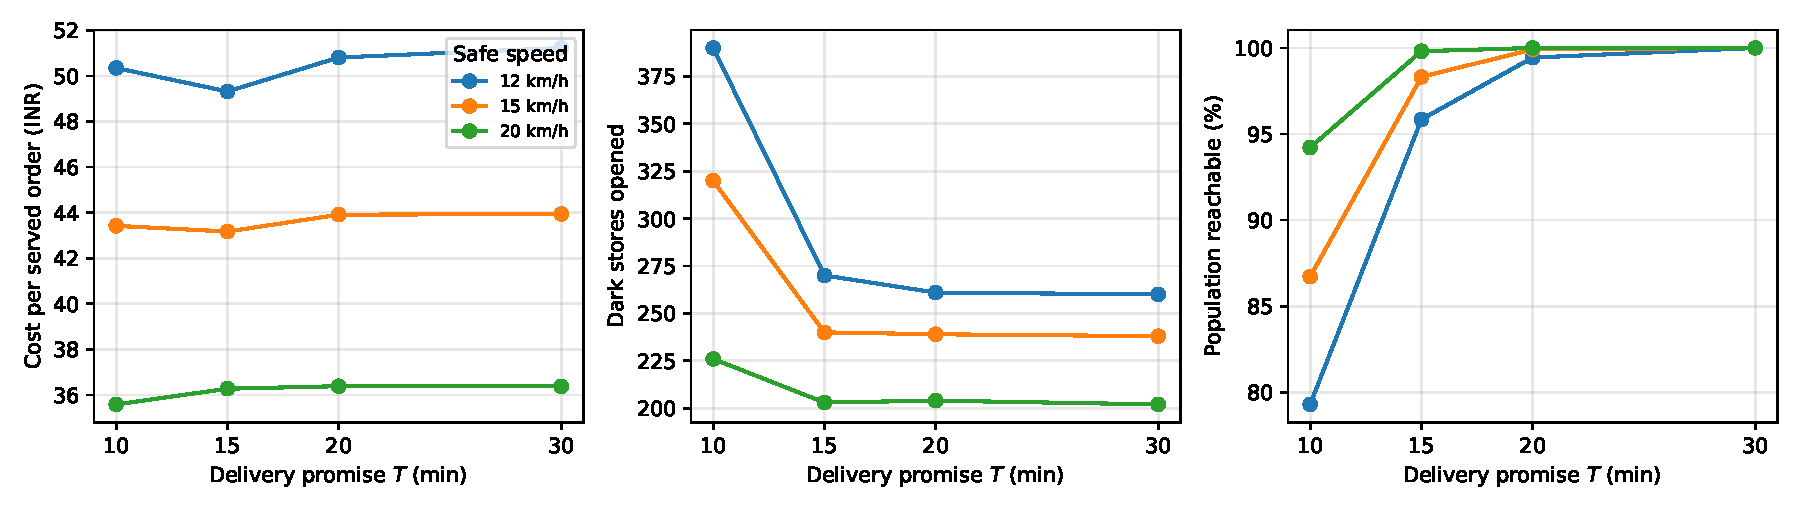
\includegraphics[width=\linewidth]{price_of_speed.pdf}
\caption{The price of speed: cost per served order, stores opened and share of residents reachable, by promise $T$ and safe rider speed $v$.}\label{fig:price}
\end{figure}

\paragraph{The promise decides \emph{who} is served, not what it costs.} At a safe speed of \BaseV~km/h, a 15-minute promise reaches \ServedFifteenPct\% of residents with \StoresTFifteen{} stores at INR~\CostPerOrderFifteen{} per order. Tightening to 10 minutes raises the store count to \StoresTTen{} but leaves \UnreachTenPct\% of residents---mostly at the city's edge, where retail stock suitable for dark stores is sparse---with no candidate site within reach (Figure~\ref{fig:maps}); the cost per served order barely moves (INR~\CostPerOrderTen{}). Relaxing the promise beyond 15 minutes changes almost nothing: the cost-optimal network has about \StoresTTwenty{} stores whether the promise is 20 or 30 minutes, because the cost trade-off between stores and rider time, not the promise, then determines the radius.

\paragraph{The speed cap decides what it costs.} Because riders are paid per logged-in hour, cost per order falls steeply with rider speed: at $T=15$ it is INR~\CostPerOrderVTwelve{} at 12~km/h, \CostPerOrderFifteen{} at 15~km/h and \CostPerOrderVTwenty{} at 20~km/h. Capping speed at 15 rather than 20~km/h costs about \SpeedCapPremiumPct\% more per order. This is the platform's economic incentive to push speed---independent of the advertised promise---and the quantity a regulator implicitly prices when it sets a speed norm.

\paragraph{The cost-optimal network is smaller than today's.} A single network serving all of Bengaluru's demand at minimum cost needs \StoreRange{} stores across the scenarios, against roughly \CurrentStores{} operated by three competing platforms today. The gap is a measure of the duplication that competition creates.

\begin{figure}[ht]
\centering
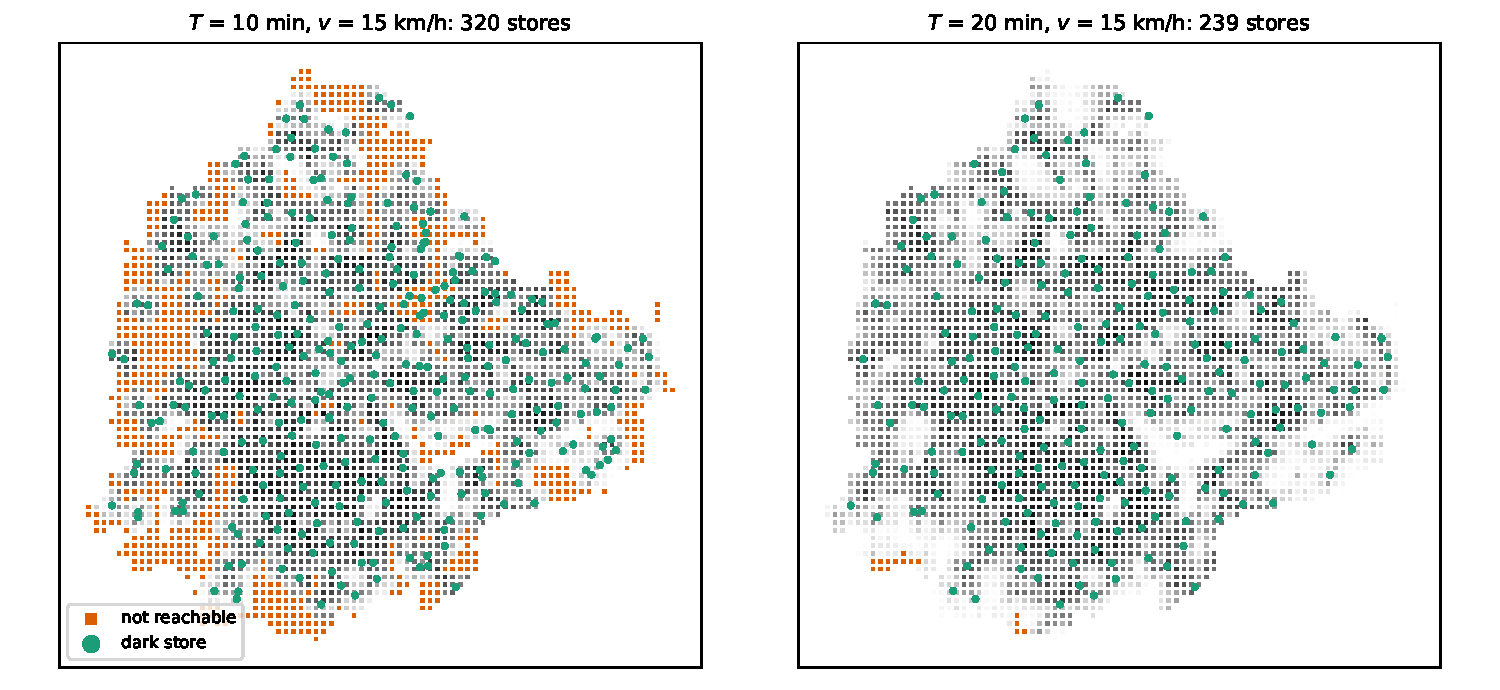
\includegraphics[width=\linewidth]{network_maps.pdf}
\caption{Optimal networks for $T=10$ and $T=20$ minutes at 15~km/h. Grey cells are served; orange cells have no candidate site within reach.}\label{fig:maps}
\end{figure}

\paragraph{The price of speed at equal coverage.} The coverage gap at $T=10$ arises because mapped retail sites are scarce at the city's edge. Allowing a store anywhere on a $\sim$0.9~km lattice of populated cells (\GridCandidates{} candidate sites), a 10-minute promise reaches \GridTenServedPct\% of residents but needs \GridTenStores{} stores at INR~\GridTenCost{} per order, against \GridFifteenStores{} stores at INR~\GridFifteenCost{} for 15 minutes. Serving \emph{everyone} within 10 rather than 15 minutes therefore needs \GridStorePremiumPct\% more stores and costs \GridCostPremiumPct\% more per order---about INR~\GridPricePerMinute{} per order for each minute saved. The price of the last five minutes is paid mainly in real estate at the periphery, which the platforms' current networks largely avoid.

\subsection{Fulfilment reliability (PERT)}

Table~\ref{tab:pert} gives the PERT estimate of fulfilment time in each network at 15~km/h. Inside the designed networks every served address is within the ride radius, so on-time probabilities are high: \PertTenP\% at $T=10$. A 10-minute promise met 95\% of the time requires riders to average \PertTenSpeed~km/h in the 10-minute network---below the safe speed. Ten-minute delivery is therefore feasible without speeding, \emph{but only} with a dense network and only for the \ServedTenPct\% of residents that network can reach.

\begin{table}[ht]
\centering\small
\caption{PERT fulfilment time by promise (network designed for that promise, $v=15$~km/h).}\label{tab:pert}
\begin{tabular}{rrrrr}
\toprule
$T$ (min) & Mean (min) & SD (min) & $P$(on time) & Speed for 95\% (km/h) \\
\midrule
10 & 7.33 & 0.99 & 0.997 & 12.1 \\
15 & 8.11 & 1.31 & 1.000 & 8.3 \\
20 & 8.23 & 1.40 & 1.000 & 6.0 \\
30 & 8.23 & 1.40 & 1.000 & 5.0 \\
\bottomrule
\end{tabular}

\end{table}

\subsection{Peak dispatch (assignment)}

The pressure appears when a network designed for one promise is asked to meet a tighter one. Table~\ref{tab:assign} dispatches a 10-minute peak batch at a stressed store of the 15-minute network (90th percentile of mean ride distance, \AssignStressRide~km). With the full sized fleet, a 15-minute promise is met for every order, but a 10-minute promise only for \AssignStressTenOnTime\%; the late orders could be saved only if riders averaged about \AssignStressSpeed~km/h, above the safe speed. Under lean staffing the gap widens sharply. Optimal assignment reduces total lateness relative to first-in-first-out dispatch, although because it minimises lateness rather than the count of late orders it occasionally delivers fewer orders strictly on time. \todo{Comment on the median store, where 60\% staffing suffices for all promises.}

\begin{table}[ht]
\centering\small
\caption{Peak 10-minute batch at a stressed store of the 15-minute network: optimal assignment vs FIFO.}\label{tab:assign}
\begin{tabular}{rrrrrr}
\toprule
Staffing & Riders & $T$ & On time & On time & Mean lateness (min) \\
 & & (min) & optimal & FIFO & optimal / FIFO \\
\midrule
40\% & 32 & 10 & 17\% & 26\% & 4.24 / 4.47 \\
40\% & 32 & 15 & 56\% & 59\% & 0.89 / 1.46 \\
40\% & 32 & 20 & 100\% & 90\% & 0.00 / 0.25 \\
60\% & 47 & 10 & 35\% & 49\% & 1.19 / 1.52 \\
60\% & 47 & 15 & 100\% & 93\% & 0.00 / 0.10 \\
60\% & 47 & 20 & 100\% & 100\% & 0.00 / 0.00 \\
80\% & 63 & 10 & 64\% & 64\% & 0.82 / 0.83 \\
80\% & 63 & 15 & 100\% & 100\% & 0.00 / 0.00 \\
80\% & 63 & 20 & 100\% & 100\% & 0.00 / 0.00 \\
100\% & 79 & 10 & 64\% & 64\% & 0.82 / 0.82 \\
100\% & 79 & 15 & 100\% & 100\% & 0.00 / 0.00 \\
100\% & 79 & 20 & 100\% & 100\% & 0.00 / 0.00 \\
\bottomrule
\end{tabular}

\end{table}

\subsection{Replenishment (transportation)}

For the base network ($T=15$, $v=15$; \StoresTFifteen{} stores), replenishment from three equal-capacity mother hubs costs \TransLP~million order-km per day at the optimum. Vogel's approximation comes within \TransVAMGapPct\% of the optimum, while the north-west corner rule is \TransNWRatio{} times worse. Supplying each store from its nearest hub would cost \TransNearest~million order-km, so equal hub capacities carry a \TransCapPremiumPct\% premium. Because the store count hardly changes beyond 15 minutes, replenishment cost is insensitive to the promise in that range.

\subsection{Sensitivity analysis}

Figure~\ref{fig:tornado} varies each uncertain input over its range at the base case. The cost per order is most sensitive to \TornadoTop{} (a swing of INR~\TornadoTopSpan) and \TornadoSecond{} (INR~\TornadoSecondSpan): rider time dominates the cost structure, which is why speed is the platform's main lever. Higher rider cost or demand raises the optimal number of stores, shortening rides; higher store cost lowers it. Longer pick-and-pack times shrink the ride radius; cost per \emph{served} order changes little because the hardest-to-serve cells drop out, which again shows that tighter time budgets are paid in coverage. The headline findings---a store count near the base case, cost flat in $T$ beyond 15 minutes, and speed as the cost driver---hold across all ranges.

\begin{figure}[ht]
\centering
\IfFileExists{figures/tornado.pdf}{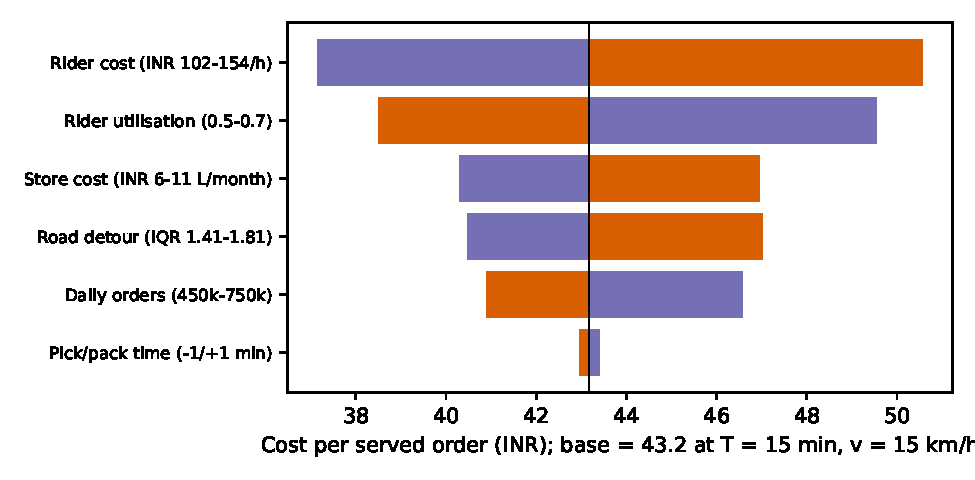
\includegraphics[width=0.85\linewidth]{tornado.pdf}}{\todo{tornado figure pending}}
\caption{One-at-a-time sensitivity of cost per served order ($T=15$, $v=15$).}\label{fig:tornado}
\end{figure}

\section{Discussion}\label{sec:discussion}

\subsection{What makes a speed target ``unrealistic''?}

The results separate two quantities that the public debate conflates. The \emph{promise} $T$ is a network-design decision: it determines how many stores are needed and which neighbourhoods can be served. The \emph{speed} riders must sustain is a cost decision: at a given network, faster riding is cheaper for the platform because rider time is paid per hour. A promise becomes unrealistic when the network cannot deliver it at a safe speed. Our results suggest a practical test for regulators: a promise is realistic for an address if the address lies within the safe ride radius of an open store after realistic pick-and-pack time---exactly the reachability set $A$ in M1. By that test, 15 minutes is realistic for \ServedFifteenPct\% of Bengaluru residents with the cost-optimal network, while 10 minutes is realistic for \ServedTenPct\% even with \StoresTTen{} stores. Promising 10 minutes beyond that footprint, or asking a 15-minute network to deliver in 10, can be met only by faster riding (Section~\ref{sec:results}).

\subsection{Managerial implications}

For platforms, the cost per order is nearly flat between 10 and 30 minutes once the network is designed for the promise; the expensive lever is rider speed. Platforms can therefore offer differentiated promises---10 minutes in dense cores, where mapped retail space allows it, and 15 elsewhere---at modest cost (a uniform 10-minute promise for everyone costs about \GridCostPremiumPct\% more per order), and should resist meeting tight promises at peaks through speed. Dispatch quality matters most at stressed stores and lean staffing, where optimal assignment reduces lateness relative to FIFO.

\subsection{Policy implications}

A speed norm is more enforceable than a promise ban. A cap of 15~km/h raises cost per order by about \SpeedCapPremiumPct\% relative to 20~km/h in our base case---a quantifiable price of rider safety that can be weighed against accident risk. Platform disclosures of delivery radius and store density would allow regulators to check reachability directly.

\subsection{Limitations}

Demand is spatialised from residential population and calibrated from platform-level disclosures rather than order data; store counts come from a third-party tracker; candidate sites depend on OpenStreetMap completeness; road distances use a single detour factor and free-flow routing; rider cost is a per-hour average; and the model represents one network rather than three competing platforms. PERT assumes independent activities and a normal approximation. \todo{Add limitations from the bibliometric part.}

\subsection{Future research agenda}

\todo{Tie each item to a gap from Section~\ref{sec:lit}.} Promising directions include competitive location models for multiple platforms, time-dependent travel times and congestion, capacity and inventory at dark stores, explicit accident-risk functions in the objective, and dynamic dispatch with fairness constraints for riders.

\section{Conclusion}\label{sec:conclusion}

\textbf{RQ1.} OR research on last-mile delivery has grown by \BibGrowthPct\% a year since 2015, led by vehicle routing with drones, robots and two-echelon systems solved by mixed-integer programming and large neighbourhood search; quick commerce (\BibQComm{} of \BibIncluded{} articles), India (none) and rider welfare (\BibWelfare) remain almost unstudied, and the delivery promise is rarely a decision variable.
\textbf{RQ2.} In Bengaluru the cost-optimal network has about \StoresTFifteen{} dark stores for any promise of 15 minutes or more; a 10-minute promise cannot reach \UnreachTenPct\% of residents from mapped retail sites, and serving everyone within 10 minutes needs \GridStorePremiumPct\% more stores at \GridCostPremiumPct\% higher cost per order. Rider speed, not the promise, drives cost: a 15~km/h cap costs about \SpeedCapPremiumPct\% more per order than 20~km/h.
\textbf{RQ3.} A promise is realistic where an address lies within the safe ride radius of a store; on that basis 15 minutes is realistic for nearly all of Bengaluru and 10 minutes for \MixedTenShare\% of residents, and a promise differentiated this way costs only \MixedPremiumPct\% more per order than a uniform 15-minute network. Regulating speed norms and disclosure of delivery radii is more meaningful than regulating advertised minutes.


\section*{Acknowledgements}
We thank Dr Vishal Pradhan, instructor of the Operations Research Management course at NMIMS University, Mumbai, for guidance throughout this project, including on the bibliometric research process. We also acknowledge the open data and software on which this study relies: map data \copyright{} OpenStreetMap contributors (ODbL~1.0), obtained via Geofabrik; WorldPop, University of Southampton, for gridded population estimates; OpenCity.in and Devdatta Tengshe for the BBMP ward boundaries; OpenAlex for bibliographic metadata; and the developers of OSRM, PuLP, HiGHS and Bibliometrix.

\bibliographystyle{plainnat}
\bibliography{references,lit}

\end{document}
